\documentclass{article}
\usepackage{graphicx}
\usepackage{epstopdf}
\usepackage{amsmath}

\title{Sparse Matrix Multiplication}
\author{Eric Jones}
\date{\today}

\begin{document}
\maketitle


\section{Introduction}

A sparse matrix consists of mostly zero-valued elements, and are prevalent
whenever connected graphs are used; or when computing some sort of physical
Hamiltonian (often tridiagonal); or when computing a PageRank. In this project,
I built code from scratch to multiply sparse matrices efficiently, and ran the
code on Mio. Ultimately, I found that my code experienced super-linear speedup,
which occurred as a result of my code implementation. \\

\section{Overview}

This project has various ways by which it can be run. First, the program can
either create a random sparse matrix or read one in from the disk. With the
sparse matrix in hand, which is currently implemented for only square $N\times N$
matrices, the program converts the matrix into an array, which retains the same
amount of information as the matrix but in a much more concise manner. Then,
these arrays are multiplied directly, allowing for the trivial
multiplications-by-zero to be avoided. From here, the matrix product can be
converted back into a full (sparse) matrix form. For my
program, I tended to use a density of around .01 (so there is one nonzero
element for every 99 zero elements).

\section{Serial Method}
\subsection{Representing Matrix as a Vector}
First, consider a matrix $A$. We can represent it as a vector of triplets
$\tilde{a}_{ij} = (i, \ j, a_{ij})$, where we only select the nonzero elements
$a_{ij}$ from $A$, so that (and similarly for B) $$\tilde{A} = \left[ \begin{tabular}{c}
    $\tilde{a}_{i_1j_1}$ \\ $\vdots$ \\ $\tilde{a}_{i_{M_A}j_{M_A}}$ \end{tabular}  
\right] \quad \quad \tilde{B}
= \left[ \begin{tabular}{c} $\tilde{b}_{k_1l_1}$ \\ $\vdots$ \\
        $\tilde{b}_{k_{M_B}l_{M_B}}$
\end{tabular}  \right],$$ 
where there are $M_{A,B}$ nonzero elements in $A$ or $B$. For sparse matrices
$M << n^2$, and so storing this vector is much more memory efficient than
storing the entire matrix. For illustration, a full matrix for $N=3000$ and 1\%
density required storage space of 105 megabytes, compared to 3.2 megabytes for 
the vector. \\

In my code's implementation, this vector representation is implemented by serially
cycling through the matrix $A$ (or $B$), and placing any nonzero element, along
with its index, into the vector $\tilde{A}$ or $\tilde{B}$. Since I am not
comfortable with pointer arrays in Fortran, the memory allocation for this
process was inefficient; I needed to search through all of $A$ to determine the
number of elements, then allocate the vector with the proper size, and only then
fill the vector with the nonzero elements of the matrix. Much of this project,
indeed, could have been more cleverly written with the use of dynamic (pointer)
arrays. 

\subsection{Sparse ``Matrix'' Multiplication}\label{sparse_mult}

From our standard matrix multiplication method, 
$$c_{i j} = \sum_{k=1}^n a_{ik} b_{kj},$$ we see that an element in C will exist
only if the inner indices of $a_{ik}b_{kj}$ match. Hence, we have a rule which
determines whether elements from our $\tilde{A}$ and $\tilde{B}$ vectors will
line up to create an element in $C$ which we can take advantage of. Using the
pseudocode $$\texttt{if $j_{R1} = k_{R2}$ then  } c_{i_{R1}l_{R2}} =
a_{i_{R1}j_{R1}}b_{k_{R2}l_{R2}},$$ where $R1$ and $R2$ are some index, 
we avoid any extraneous multiplications by following this method;
since $A$ and $B$ are sparse, $C$ tends to be as well, and so this algorithm is
more efficient than our standard (na\"{i}ve) matrix multiplication
implementation. In essence, this sparse matrix multiplication uses that if the
inner indices of elements in $\tilde{A}$ and $\tilde{B}$ match, then there will
be a resulting element in $C$, with its index being the outer indices of the two
elements of $\tilde{A}$ and $\tilde{B}$. \\

However, sometimes there are multiple elements that contribute to the value of a
given element of $C$, which can overwrite other elements if we're not careful.
To remedy this, before appending any new element to $C$ we check through all of
$C$ to see whether the new element has been calculated before. If the element
already exists, the old value is incremented by the new value; if the element
doesn't exist, it is created. By this method, we ensure that no elements are
overwritten or omitted from the final calculation. 

\section{Parallel Implementation}\label{parallel}
\subsection{Sorting the Matrix}
In the scheme by which I've performed sparse matrix multiplication for this
project, the vector need to be sorted in order to be parallelized.  This sorting
is incredibly useful towards performing the sparse matrix multiplication, and is
one of the key components in the super-linear speedup acquired when running this
code in parallel (as will be discussed in Section \ref{results}). \\

Sorting is necessary to parallelize the code, at least in the current scheme, as
each processor needs to be passed subvectors of $\tilde{A}$ and $\tilde{B}$
which have elements which are able to be multiplied together. To this end, I
sort the vector $\tilde{A}$ by the $j$ index, and sort vector $\tilde{B}$ by the
$i$ index, which (as described in Section \ref{sparse_mult}) allows for a clear
distribution of the vector among processors. \\

However, sorting these vectors ended up being quite a task in itself. As sorting
was not the focus of my project, I did not parallelize it and expected that this
section would occupy a small portion of the run-time. However, my sorting method 
selection sort has order $\mathcal{O}(N^2)$ complexity, which scales poorly with
the problem. If I were to approach this project a second time, I would use a
precoded library of some sort like quicksort, which would surely improve
computation time. As a side note, in the future I would like to implement some
parallelized sorting method, as it seems like a somewhat intriguing problem. \\

The outcome of this computational complexity is that the time required to sort
the vectors takes around the same amount of time as the matrix multiplication in
serial requires, as will be discussed in Section \ref{results}. In computing the
time required for this code to run, I avoided considering the (dominating) time
required to sort. 

\subsection{Distributing $\tilde{A}$ and $\tilde{B}$ to Processors}
To start, each processor was broadcast the whole of $\tilde{A}$ and $\tilde{B}$,
and so they were able to manipulate this vector to arrive at their respective
subvector used in the parallel sparse multiplication. In future versions, I
would like to be more memory efficient by only having each processor hold the
information they need initially.\\

We give each processor a subvector of triples corresponding to a range of $j$ of
length $\texttt{floor}\left(\frac{n}{P}\right)$. For example, consider when
$n=8$, $P=4$, and $\tilde{A}$; in this case, each processor is allocated
elements spanning $2$ $j$-indices:  $$ \tilde{A} = [ \
    \underbrace{\tilde{a}_{3,1}, \  \tilde{a}_{8,1}, \ \tilde{a}_{2,2}, \
    \tilde{a}_{3,2}}_\text{proc 1}, \ \overbrace{\tilde{a}_{6,4}}^\text{proc 2},
    \ \underbrace{\tilde{a}_{1,5}, \ \tilde{a}_{1,6}, \
\tilde{a}_{7,6}}_\text{proc 3}, \ \overbrace{\tilde{a}_{2,7}, \
\tilde{a}_{7,7}}^\text{proc 4} \ ]$$ We pass processors triples for $B$ in a
similar way, corresponding to a range of the $i$-index. From this, the
processors will only have elements from $\tilde{A}$ and $\tilde{B}$ which match
and can be multiplied yield elements of $C$.\\

In distributing the vectors among processors, I first sorted the vectors as
above. Then, I created an index based on the sorted vector, documenting which
elements corresponded to which $i$ or $j$ index. From this index, the
distribution of triples among cores was relatively simple. 

\subsection{Parallel Sparse Matrix Multiplication}
Now, since each processor has a subvector of $\tilde{A}$ and $\tilde{B}$, they
are able to multiply the two together in precisely the same way as explained in
the serial implementation in Section \ref{sparse_mult}. The modularity of this
sparse matrix multiplication subroutine allows for it to be used in serial or in
parallel. From this, each processor computes a subvector of $C$, and passes each
constituent to the master core: for this, I created a new datatype
\texttt{MPI\_TRIPLE} which I then used to pass the $C$ subvectors
using \texttt{MPI\_Gather}. \\

The gathered $C$ matrix may still contain duplicates, as during the parallel
multiplication the processors don't talk to each other, so as a final step the
$C$ matrix is ``flattened,'' where multiples of elements are consolidated into one
entry. 

\subsection{Output}
For small cases, I was able to ``clean up'' the resultant matrices and present
them in a readable form, but for large matrices this cleaning process was
extremely inefficient.  For small matrices---used specifically to show the
legitimacy of this matrix multiplication---the extra zero elements (required
since I didn't use pointer arrays) padding the vector are removed, and the
matrix is printed to the screen. 

\section{Results \label{results}}
Due to the computational expense of sorting the vectors, the running of this
code on Mio is different from the running of this code in general. In the
directory of files, there is one directory to run the code for small matrices
(e.g. $N=10$) and another directory meant for running on Mio for large matrices
(e.g. $N=3000$). \\

When running the code on Mio, to avoid sorting the vectors each time, I had one
processor create two large sparse matrix and sort each into a vector, and then save
these data structures to the disk. The other processors simply read these
structures from the disk, allowing for all of their time to be spent computing
the sparse matrix multiplication. \\

In the following figures, we are benchmarking only the part of parallelization
required to multiply the matrices. This means that we do not take into account
the time required to sort the vectors, or the time required to make the output
look ``neat.'' We do take into account the reading of matrices and vectors from
disk, the distribution of vectors among cores, the sparse matrix multiplication,
and the collection of each processor's subvectors of $C$. Of these tasks, the
sparse matrix multiplication takes the vast majority of the time ($\sim 99\%$
for large matrices). \\

For these plots, I used a matrix where $N=3000$ and the density of the matrices
was .01. I ran the sparse matrix multiplication on the same two matrices for
$P=2^k, \ k=0,  \ldots,  6$. 

\begin{figure}
\centering
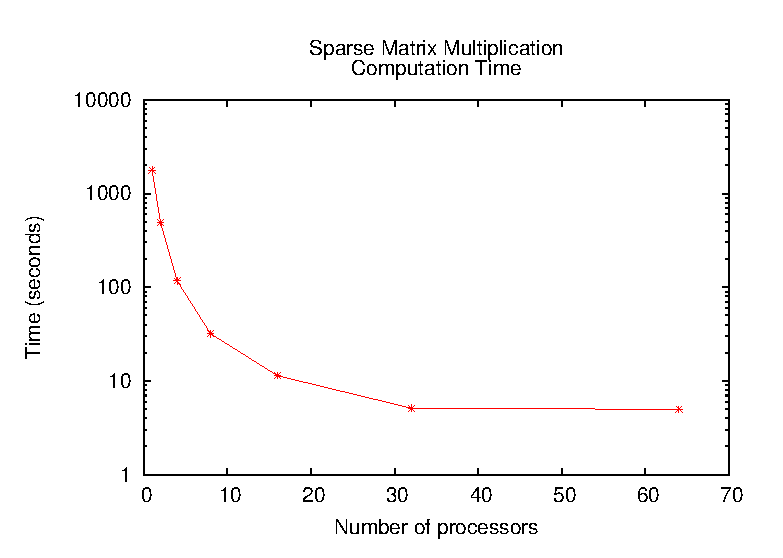
\includegraphics[width=0.7\textwidth]{time_plot_3000.eps}
\caption{\label{time} Time required to run code for a representative sparse
matrix muliplication over $2^k, k=0,\ldots,6$ processors.}
\end{figure}

\begin{figure}
\centering
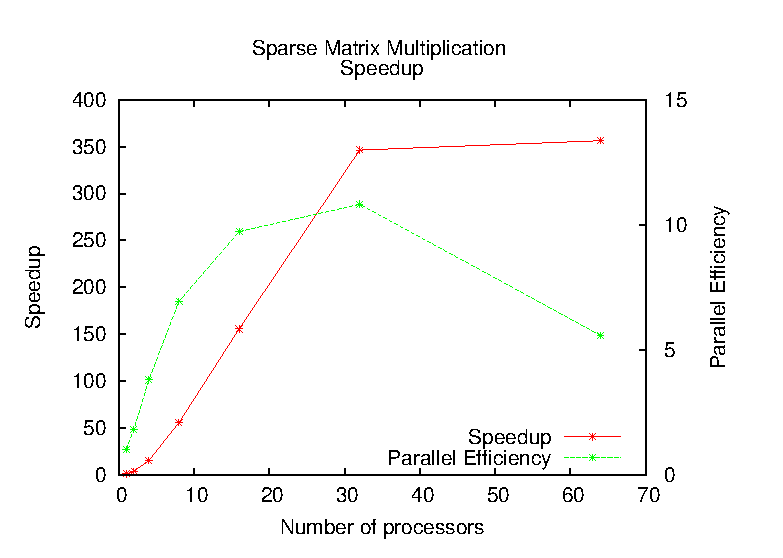
\includegraphics[width=0.7\textwidth]{speedup_plot_3000.eps}
\caption{\label{speedup} Speedup for a representative sparse
matrix muliplication over $2^k, k=0,\ldots,6$ processors.}
\end{figure}

\begin{figure}
\centering
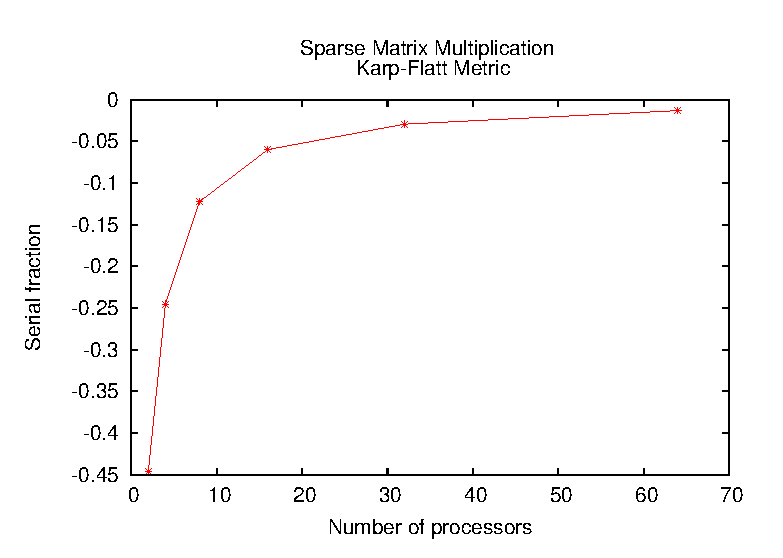
\includegraphics[width=0.7\textwidth]{karp_plot_3000.eps}
\caption{\label{karp} Karp-Flatt serial fraction over a representative sparse
matrix muliplication over $2^k, k=0,\ldots,6$ processors.}
\end{figure}

\begin{table}[h]
    \centering
\begin{tabular}{|l|l|l|l|l|} \hline
    Processors & Time (s) & Speedup & Efficiency & Serial fraction \\ \hline
\hline    1          & 1771.634 & 1.000   & 1.000      &                 \\
    2          & 490.342  & 3.613   & 1.807      & -0.446          \\
    4          & 116.873  & 15.159  & 3.790      & -0.245          \\
    8          & 31.937   & 55.473  & 6.934      & -0.122          \\
    16         & 11.378   & 155.703 & 9.731      & -0.060          \\
    32         & 5.114    & 346.413 & 10.825     & -0.029          \\
    64         & 4.970    & 356.448 & 5.570      & -0.013         \\ \hline
\end{tabular}
\caption{Parallel performance of this code on Mio \label{table}}
\end{table}

\subsection{Analysis of Results}
My results (seen in Table \ref{table}) are a little strange- I have well over super-linear speedup (closer
to quadratic speedup), with efficiencies larger than 1, and a negative serial
fraction. The reason for each of these strange metrics is due to the
implementation of my parallel sparse multiplication, and the $\mathcal{O}(n^2)$
complexity hidden within the multiplication. \\

When I perform the pseudocode above, which finds compatible elements in
$\tilde{A}$ and $\tilde{B}$ which result in an element in $C$, the algorithm
scans through all of $\tilde{B}$ for each element of $\tilde{A}$, resulting in a
quadratic complexity. As I double the number of processors, I halve the
number of elements in each processor's subvector, which takes a quarter of the
time to search. It is due to this that my performance metrics are unusual, since
the metrics are typically applied to problems that stay the same when broken up
into pieces (e.g. summing a series of numbers) versus my case, where breaking up
the program into pieces inherently increases the performance of each processor,
as well as the speedup gained by parallelizing the process.

\subsection{Metrics}
I have provided the speedup $S_P$, $T_1/T_P$, which gives how much faster the
processor performs in parallel versus in serial. For my program, speedups were
on the order of $P^2$ where $P$ is the number of processors. As mentioned above,
this is consistent with the expected performance, as making the subvectors
contain fewer elements results in a faster searching time. In addition, I
considered the parallel efficiency $E_P$, $S_P/P$, which was always greater than
1. Still, the efficiency tapered off between 32 and 64 processors, which may be
a sign that at that point adding processors has diminishing returns. \\

Lastly, I considered the Karp-Flatt metric $f_P$, $$f_P = \frac{\frac{1}{S_P} -
\frac{1}{P}}{1-\frac{1}{P}},$$ which is negative for my program. This is due to
the numerator, as for my results $S_P > P$ which will result in a negative
numerator. We see that in the limit, $$\lim_{P\to \infty}f_P = 0,$$ as expected.

\section{Conclusion}
In the course of this project, I further defined things that I would like to
learn and plan to learn in parallel programming. First, the ability to
dynamically allocate memory would be very useful in projects like this, where
the size of vectors is unknown until the calculation is performed (the number of
nonzero elements in $C$, for example). Next, the sorting performed in this
programming ended up being the most time-consuming part of the code! This has
encouraged me to consider how to implement sorting in parallel, a task which I
would like to pursue whenever I next have free time. \\

I had hoped to parallelize my code using GPUs, but unfortunately I didn't have
the time to dedicate to this addition. I feel like sparse matrix multiplication
would be an effective use of GPU, since each processor will need memory
sufficient to store the matrix, and then just perform multiplications of the
same type. These multiplications will be the same each time, and so a GPU would
be calculate the products efficiently. At a later date, I hope to practice
parallelization with CUDA so I can take advantage of the massive GPU
speedups. \\

This project gave unexpected results for the performance metrics I used.
These peculiarities of my results forced me to consider the internals of the
parallelization, which improved my understanding of how parallelization works. I
found it interesting that parallelization could be used to inherent make the
calculations each processor makes easier, and then on top of that also
distribute the computation among processors. This two-fold increase in
efficiency makes me curious in what other ways parallelization can be sped up,
simply by the code structure used. \\

In further work, I would like to consider different metrics which I could use
for my code, which take into account the fact that as a parallelize between more
processors, each processor's piece is inherently easier to compute. I was
considering creating a ``quadratic efficiency,'' $QE_P=\frac{S_P}{P^2}$, which
might give results more similar to those I've seen before; whether these metrics
have any merit, though, would be a project in itself. 



\end{document}
